\documentclass{article}
\usepackage[utf8]{inputenc}

\usepackage[margin=1in]{geometry}
\usepackage{hyperref}
\usepackage{graphicx}
\usepackage{ulem}

\usepackage{titlesec}
\setcounter{secnumdepth}{4}
\setcounter{tocdepth}{4}
\titleformat{\paragraph}
{\normalfont\normalsize\bfseries}{\theparagraph}{1em}{}
\titlespacing*{\paragraph}
%{0pt}{3.25ex plus 1ex minus .2ex}{1.5ex plus .2ex}
{0pt}{1.0ex plus 1ex minus .2ex}{0.1ex plus .2ex}

\newcommand{\name}{ECW\ }
\newcommand{\nameNospace}{ECW}
\newcommand{\namep}{ECW.}

\renewcommand{\labelenumii}{\theenumii}
\renewcommand{\theenumii}{\theenumi.\arabic{enumii}}
\renewcommand{\theenumiii}{\theenumii.\arabic{enumiii}}

\usepackage{fancyhdr}
\pagestyle{fancy}

\lhead{ Responsible: Alexander Ekman \& Linnea Johnsson \\ Date: \today}  \rhead{Document number: PRD \\ Version: 1.0}
\renewcommand{\headrulewidth}{0.5pt} 



\title{PRD - Product Requirements Document}
%\title{Submodule test}
%\title{Submodule test2}
\author{Team 1}

\begin{document}

\date{}
\maketitle
\thispagestyle{fancy}
\newpage

\tableofcontents
%\newpage

\section*{Revision history}
%\begin{center}
\begin{tabular}{ |c|c|l| } 
 \hline
 Version & Date & Reason \\ \hline
 1.0 & 2021-09-15 & First draft \\ 
 1.1 & 2021-09-15 & Fixed typos from team feedback \\ 
 1.11 & 2021-09-20 &  Added SDP and PH book to reference documents\\
 \hline
\end{tabular}
%\end{center}

\newpage
\section{Feedback}
\begin{itemize}
    \item 11: \sout{In section "revision history": Were there earlier versions of the document, that were revised per the team members' feedback?}
    \item 14: In section 2:
    \begin{itemize}
        \item Move referenced documents section before Introduction section.
        \item Reference PH Book (Uppdragbeskrivning)
        \item Reference SDP
    \end{itemize}
    \item 15: section 1: Reference PH Book Chapter 9
    \item 16: section 3.2: Admin user not discussed
    \item 17: section 4: Admin user not discussed
    \item 18: Section 5:
    \begin{itemize}
        \item -Please do not deviate from UML standard when creating system use case diagram. You can draw by hand, use limited free version of Omni Graffle, StarUML... Please see example in exercise 1.2. Take advantage of <<uses>> tag.
        \item Can Driver and Rider edit registered ride request or trip?
        \item Can Driver edit vehicle information?
    \end{itemize}
    \item 20: section 7.2: Connect requirements to user stories
    \item 21: section 7.2.1 Which non-functional requirement characteristic can requirements under 7.3 section be grouped under (performance, reliability, usability, portability...)? Can you add more non- functional requirements?
    \item 22: Which technology will you be using (Base system server...) Development ID, any test suites (e.g. Junit), version control (Gitlab)... ?
    \item 24: Discuss the destinations given in BASE?
    \item 25: SPF1: Prioritize issues
    \item 26: SP1: Something was discussed
\end{itemize}

Questions
\begin{itemize}
    \item What are we supposed to reference from the SDP in the PRD?
\end{itemize}

\newpage

\section{Referenced documents}
\begin{thebibliography}{widest entry}
    \bibitem{BNL} "Ride sharing Benefits, Brooklyn National Laboratory", 2012, url=\url{https://www.bnl.gov/rideshare/benefits.asp}, accessed 2021-09-14
    
    \bibitem{PH} "Programvaruutveckling för Stora System Projekthandledning 2021", Institutionen för Datavetenskap Lunds Tekniska Högskola, Lunds Universitet, 26 August 2021
    
    \bibitem{SDP} "SDP - Software Development Plan, Team 1 - ETSN05", Alexander Ekman and Linnea Johnsson, url=\url{https://www.overleaf.com/read/bvbkjmdrkpdx}, accessed \today
    
\end{thebibliography}

\section{Introduction}
This Product Requirements Document (PRD) details the requirements to develop a web-app based carpool service called ETSN05\_PG1 Carpool Webb-app (\nameNospace).

The purpose of this PRD is to provide the system characteristics, the epics and user stories, as well as the requirements of the system. This document is intended as a basis for the contract between the development team and the client, it will also serve as a reference for the development team during the development process.

\section{Background and product goals}
\subsection{Purpose}
A lot of the cars on our roads today are only transporting single individuals, which is problematic when aiming for a more sustainable future ~\cite{BNL}. The goal of \name is to give non-car owners and car owners the ability to easily match with each other and carpool together to a common destination. \name will provide its users with a more economic and sustainable mode of transportation.

\subsection{System Users}
The system user is either a non-car-owner who would like to carpool somewhere (rider), a car owner who is willing to bring someone along a planned route (driver), or someone who sometimes is a driver and sometimes a rider.

\name users will register an account as either driver, rider or both. A rider can log in and request a stating city, a destination city, and a time and date they would like to go. Likewise, a driver can submit a starting city, a destination and a time that they have planned to leave, and if a drivers submission matches with one or several riders requests a match is made. Contact details are then shared between the users for easy communication between them. All users are also here given the option to decline the offer. For future versions it is planned for drivers to be able to enter multiple cities where they are willing to stop, and in such a way be able to support more short distance riders.

\section{Terminology}
\name = The name of the system\newline
Driver = A car owner who is willing to bring someone along a planned route\newline
Rider = A non-car-owner who would like to carpool somewhere\newline
Drive instance = The objects created when a driver has declared that they will be driving a certain route a certain date and time
Ride request = The objects created when a rider has declared that they would like to ride along a certain route a certain date and time

\newpage
\section{System Use Case Diagram}
\begin{figure}[!htpb]
    \centering
    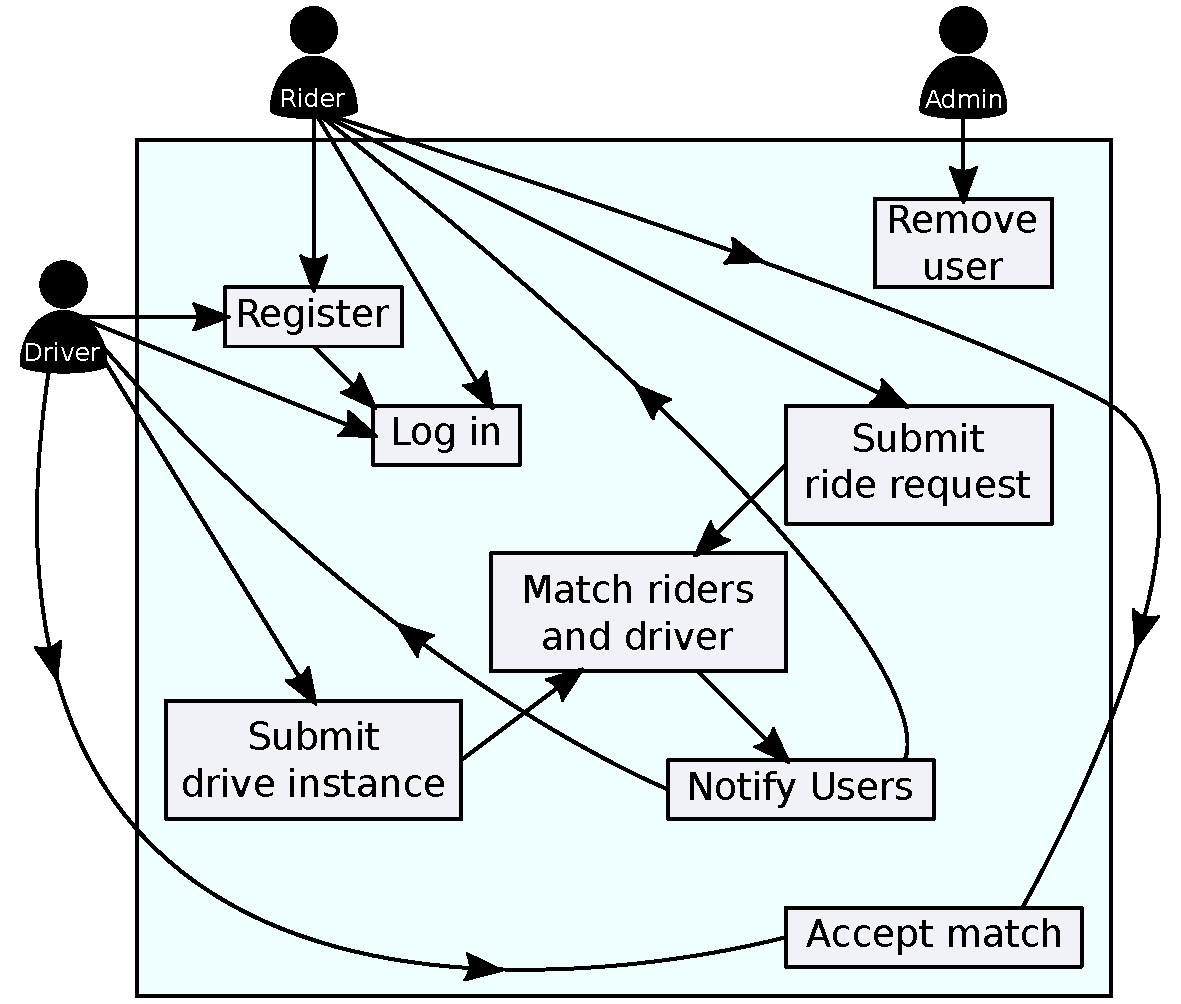
\includegraphics[scale=0.75]{system_case_diagram.pdf}
    \caption{The system use case diagram for \namep. Users register as either drivers, riders, or both and can after registration log in to access the service. A driver submits a an origin, destination, and time. If a rider has a similar request a match is made and the users are notified. The users can then accept or decline the match.}
    \label{fig:useCaseDiagram}
\end{figure}

\newpage
\section{Epics, User stories, and Issues}
The entries are labeled as X.Y.Z where this represents a unique identifier as Epic.Story.Issue.
\begin{enumerate}
  
  \item User registration and authentication
  \begin{enumerate}
    \item As a user, I can register for the service as rider, drivers, or both
    \begin{enumerate}
        \item All users register full name, email, and phone number
        \item If a user is a driver, they register car brand, model, color, and licence plate
        \item Design registration window
        \item Add a registration button in the login window
        \item Add functionality to the registration button
        \item As a registered user, I want to be able to log in and out
        \item Users log in using email
    \end{enumerate}
  \end{enumerate}
  
  \item Matching
  \begin{enumerate}
      \item As a driver/rider, I select two cities and a time
      \begin{enumerate}
          \item If a user is registered as “both”, they have to specify if riding or driving
          \item Add a drop-down button of available cities (frontend)
          \item Add functionality to the drop-down of available cities (backend)
          \item Add a “Create Drive Instance”/“Create Ride Request” button for drivers/riders respectively (frontend)
          \item Design how to store the drive instances and ride requests
          \item If a request is created by a user it is added to the requests list
      \end{enumerate}
      \item As a driver I can also add cities on my route
  \end{enumerate}
  
  \item Matchmaking system
  \begin{enumerate}
      \item As a user, if two users have matching routes, we want to be paired up
      \begin{enumerate}
          \item Matches are made when there exists a driving instance, and there exists a rider request for a part of that route.
      \end{enumerate}
  \end{enumerate}
  
  \item After successful match
  \begin{enumerate}
      \item As a user, when a match is made, I want to be notified about the match and know how to recognize/contact each other
      \begin{enumerate}
          \item Implement notifications in BASE
          \item Send notifications to specific user
          \item Send notifications to users from match making system
          \item Include useful information in notifications (car brand, model, color, driver/rider phone number)
      \end{enumerate}
      \item As a driver, I want to be able to decline a match
      \item As a rider, I want to be able to decline a match
  \end{enumerate}
  
  \item Administration
  \begin{enumerate}
      \item As administrator I can remove users
      \begin{enumerate}
          \item Allow administrator to remove users
      \end{enumerate}
  \end{enumerate}
  
\end{enumerate}

\newpage
\section{Project Requirements}
This section contains all the functional and non-functional requirements of the system.

\subsection{Development environment}
This section contains the requirements for developing the system.

\subsubsection{Server}

\paragraph{Host}\label{req:server}
\textbf{ID}: D1\newline
\textbf{Priority}: HIGH\newline
\textbf{Description}: This project requires a server to host the web-app.\newline
\textbf{Rationale}: So that there is a website for the web-app\newline
\textbf{Dependency}: NA

\paragraph{HTML, CSS, and JavaScript}\label{req:hostingLogin}
\textbf{ID}: D2\newline
\textbf{Priority}: HIGH\newline
\textbf{Description}: This project requires a server to host HTML, CSS, and JavaScript for the user to interact with the system.\newline
\textbf{Rationale}: In order for users to use the system\newline
\textbf{Dependency}: \ref{req:server}

\paragraph{Registered users and login}\label{req:hostingLogin}
\textbf{ID}: D3\newline
\textbf{Priority}: HIGH\newline
\textbf{Description}: This project requires a server to host login details and profile information from the registration.\newline
\textbf{Rationale}: In order to have user logins and keep profile information\newline
\textbf{Dependency}: \ref{req:server}

\paragraph{Trip database}\label{req:tripDatabase}
\textbf{ID}: D4\newline
\textbf{Priority}: HIGH\newline
\textbf{Description}: This project requires a server to host the submitted ride requests and drive instances so that these can be matched.\newline
\textbf{Rationale}: In order to run a matching algorithm\newline
\textbf{Dependency}: \ref{req:server}

\paragraph{Trip matching algorithm}\label{req:matchAlgorithm}
\textbf{ID}: D5\newline
\textbf{Priority}: HIGH\newline
\textbf{Description}: This project requires a server to run the matching algorithm between submitted ride requests and drive instances so that these can be matched.\newline
\textbf{Rationale}: In order to match riders and drivers\newline
\textbf{Dependency}: \ref{req:tripDatabase}


\subsection{Functional requirements}
This section contains the requirements which specify the functions of the system.


\subsubsection{User registration and authentication}

\paragraph{User registration}\label{req:registration}
\textbf{ID}: F1\newline
\textbf{Priority}: HIGH\newline
\textbf{Description}: A prospective user should be able to access the website and be guided to registering a new account, as shown in Figure \ref{fig:login}. To register for the service, all users must provide full name, email, password, and phone number as shown in Figure \ref{fig:register}.\newline
\textbf{Rationale}: In order for new members to register for the service\newline
\textbf{Dependency}: NA

\paragraph{Driver registration}\label{req:driverRegistration}
\textbf{ID}: F2\newline
\textbf{Priority}: HIGH\newline
\textbf{Description}: A prospective user registering as a driver, or a rider and a driver must also register car brand, model, color, and licence plate number. This will be in addition to what is shown in Figure \ref{fig:register}\newline
\textbf{Rationale}: So that the driver is easily identifiable when picking up riders\newline
\textbf{Dependency}: \ref{req:registration}\newline

\paragraph{User log-in}\label{req:log-in}
\textbf{ID}: F3\newline
\textbf{Priority}: HIGH\newline
\textbf{Description}: A registered use should be able to log in using their email and password as shown in Figure \ref{fig:login}. \newline
\textbf{Rationale}: In order to submit a drive instance or a ride request\newline
\textbf{Dependency}: \ref{req:registration}\newline

\paragraph{User log-out}\label{req:log-out}
\textbf{ID}: F4\newline
\textbf{Priority}: HIGH\newline
\textbf{Description}: A logged in user should be able to log out from the current session, as shown in Figure \ref{fig:submission}. \newline
\textbf{Rationale}: In order to close a session\newline
\textbf{Dependency}: \ref{req:log-in}\newline

\subsubsection{Submitting drive instance or ride request}

\paragraph{Drive instance submission}\label{req:driveInstance}
\textbf{ID}: F5\newline
\textbf{Priority}: HIGH\newline
\textbf{Description}: A logged in driver should be able to submit a drive instance by selecting an origin, a destination, and a time and date for departure as shown in Figure \ref{fig:submission}. \newline
\textbf{Rationale}: In order to show that a car is available on this route at this time\newline
\textbf{Dependency}: \ref{req:log-in}\newline

\paragraph{Ride request submission}\label{req:rideRequest}
\textbf{ID}: F6\newline
\textbf{Priority}: HIGH\newline
\textbf{Description}: A logged in rider should be able to submit a ride request by selecting an origin, a destination, and a time and date for departure as shown in Figure \ref{fig:submission}. \newline
\textbf{Rationale}: In order to show that someone wants a ride on this route at this time\newline
\textbf{Dependency}: \ref{req:log-in}\newline

\paragraph{Dual user submission}\label{req:dualSubmission}
\textbf{ID}: F7\newline
\textbf{Priority}: MEDIUM\newline
\textbf{Description}: A logged in user registered as both rider and driver should be able to submit either a ride request or diver instance by specifying if they are driving or riding as shown in Figure \ref{fig:submission}. \newline
\textbf{Rationale}: In order for driver and rider users to specify which type of user they are for this submission\newline
\textbf{Dependency}: \ref{req:log-in}\newline

\subsubsection{User profiles}

\paragraph{Profile details}\label{req:profileDetails}
\textbf{ID}: F8\newline
\textbf{Priority}: MEDIUM\newline
\textbf{Description}: A logged in user should be able to see and edit some of their profile details as shown in Figure \ref{fig:profile}. \newline
\textbf{Rationale}: In order for users to update their details in case they change\newline
\textbf{Dependency}: \ref{req:log-in}\newline

\paragraph{Upcoming travel}\label{req:upcomingTravel}
\textbf{ID}: F9\newline
\textbf{Priority}: HIGH\newline
\textbf{Description}: A logged in user who is matched with a rider/driver should see the upcoming routes and details of that route on their profile page as shown in Figure \ref{fig:profile} and Figure \ref{fig:profile2}. \newline
\textbf{Rationale}: So that users can be reminded of the details of upcoming routes\newline
\textbf{Dependency}: \ref{req:profileDetails}\newline

\paragraph{Necessary contact details}\label{req:contactDetails}
\textbf{ID}: F10\newline
\textbf{Priority}: HIGH\newline
\textbf{Description}: Upcoming routes should display contact details of that route on the users profile page as shown in Figure \ref{fig:profile2}. \newline
\textbf{Rationale}: So that the driver and rider can find each other\newline
\textbf{Dependency}: \ref{req:profileDetails}\newline

\paragraph{Upcoming travel}\label{req:upcomingTravel}
\textbf{ID}: F11\newline
\textbf{Priority}: MEDIUM\newline
\textbf{Description}: A logged in user who is matched with a rider/driver needs to accept or decline matches with riders/drivers as shown in Figure \ref{fig:profile}. \newline
\textbf{Rationale}: In case the situation changes or the driver thinks that too many extra stops have been added\newline
\textbf{Dependency}: \ref{req:upcomingTravel}\newline

\subsubsection{User notification}

\paragraph{Match notification}\label{req:matchNotification}
\textbf{ID}: F12\newline
\textbf{Priority}: MEDIUM\newline
\textbf{Description}: When a user is matched with a driver/rider they should be notified in the web app as shown in Figure \ref{fig:submission} and Figure \ref{fig:profile3}. \newline
\textbf{Rationale}: So that users don't miss successful matches\newline
\textbf{Dependency}: \ref{req:profileDetails}\newline

\subsubsection{Web-app administration}

\paragraph{Admin log in}\label{req:adminLog-in}
\textbf{ID}: F13\newline
\textbf{Priority}: HIGH\newline
\textbf{Description}: As administrator of the system I should be able to log in and obtain extra privileges as administrator. \newline
\textbf{Rationale}: So that users abusing the system or who want to be removed can be removed\newline
\textbf{Dependency}: \ref{req:log-in}\newline

\paragraph{Removing users}\label{req:removingUser}
\textbf{ID}: F14\newline
\textbf{Priority}: HIGH\newline
\textbf{Description}: A logged in administrator should be able to remove users. \newline
\textbf{Rationale}: So that users abusing the system or who want to be removed can be removed\newline
\textbf{Dependency}: \ref{req:registration}\newline


\subsection{Non-functional requirements}
This section contains descriptions of requirements on the user interaction and system performance.


\subsubsection{Log in}

\paragraph{Entering correct username and password}\label{req:}
\textbf{ID}: NF1\newline
\textbf{Priority}: MEDIUM\newline
\textbf{Description}: A user who enters a correct username and password, once pressing the "log in" button, should not wait longer than 2 seconds to see the submission page shown in Figure \ref{fig:submission}\newline
\textbf{Rationale}: Users should not wait to long to use the service\newline
\textbf{Dependency}: \ref{req:log-in} \newline

\paragraph{Entering incorrect username and password}\label{req:}
\textbf{ID}: NF2\newline
\textbf{Priority}: MEDIUM\newline
\textbf{Description}: A user who enters an incorrect username and password, once pressing the "log in" button, should not wait longer than 2 seconds to be prompted for another attempt \ref{fig:submission}\newline
\textbf{Rationale}: Users should not wait to long to use the service\newline
\textbf{Dependency}: \ref{req:log-in} \newline


\subsubsection{User notifications}

\paragraph{Notification of new match}\label{req:}
\textbf{ID}: NF3\newline
\textbf{Priority}: LOW\newline
\textbf{Description}: After a driver/rider is matched, their profile pages should update accordingly within 10 seconds\newline
\textbf{Rationale}: Avoiding clashes in user actions\newline
\textbf{Dependency}: \ref{req:matchNotification} \newline


%\paragraph{}\label{req:}
%\textbf{Description}: \newline
%\textbf{Rational}: \newline
%\textbf{Dependency}: \newline

\newpage
\section{Appendix A: Prototypes}
\begin{figure}[!htpb]
    \centering
    \begin{minipage}{0.25\textwidth}
        \centering
        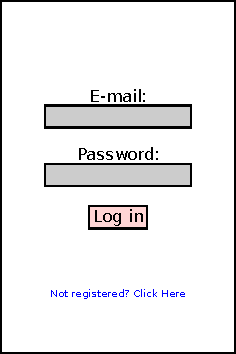
\includegraphics[scale=1]{login.pdf}
        \caption{Log-in screen shown to unauthenticated user. The window also guides unregistered users to register}
        \label{fig:login}
    \end{minipage}\hfill
    \begin{minipage}{0.25\textwidth}
        \centering
        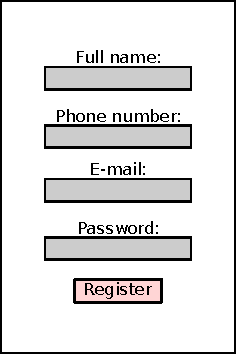
\includegraphics[scale=1]{register.pdf}
        \caption{Screen shown to users registering for the first time. A distinction will be made if they register as drivers, as specified in paragraph \ref{req:driverRegistration}}
        \label{fig:register}
    \end{minipage}\hfill
    \begin{minipage}{0.25\textwidth}
        \centering
        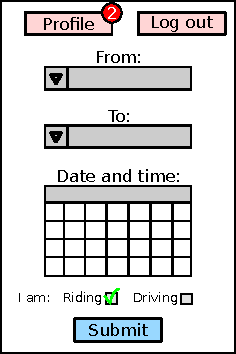
\includegraphics[scale=1]{submission2.pdf}
        \caption{Submission screen shown after successful log-in. Here riders can submit ride requests, and drivers submit drive instances}
        \label{fig:submission}
    \end{minipage}\hfill
\end{figure}

\begin{figure}[!htpb]
    \centering
    \begin{minipage}{0.25\textwidth}
        \centering
        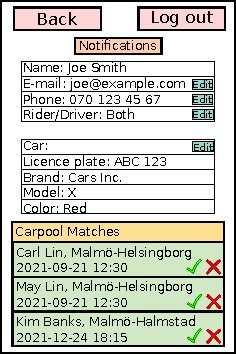
\includegraphics[scale=1]{profile.pdf}
        \caption{Profile screen showing users their current details and which of these are editable. It also shows upcoming trips and the choice to accept/decline them}
        \label{fig:profile}
    \end{minipage}\hfill
    \begin{minipage}{0.25\textwidth}
        \centering
        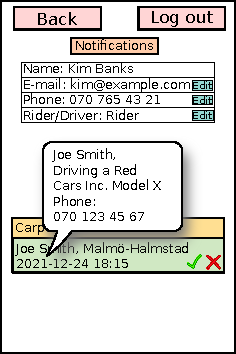
\includegraphics[scale=1]{profile2.pdf}
        \caption{Demonstration of how each upcoming trip can display more information}
        \label{fig:profile2}
    \end{minipage}\hfill
    \begin{minipage}{0.25\textwidth}
        \centering
        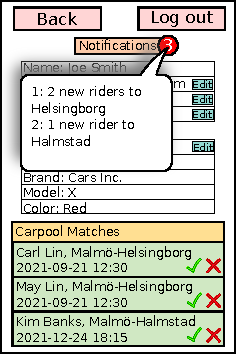
\includegraphics[scale=1]{profile3.pdf}
        \caption{Demonstration of how users will be notified about new events}
        \label{fig:profile3}
    \end{minipage}\hfill
\end{figure}

\newpage
\section{Appendix B: Route functionality}
The core functionality of this web-app is to allow drivers and riders to carpool on a common route. In order to increase the value stream to our client, we choose to prioritize this core functionality over any "smart" features such as route optimization.

As a balance between core functionality and the development teams available resources, we envision three phases of the route implementation. The first phase involves the driver specifying two cities, one origin and one destination. If these match those of a rider then there is a match. In phase two we plan to allow drivers to enter an origin, a destination, as well as stops in between which they personally consider as reasonable stops along the way. This is because adding destinations to a route seems like a solvable programming problem, but to know weather it makes sense to pick someone up in Lund on a trip from Malmö to Helsingborg (a 17 minute detour, 34\% longer) is a completely different issue than route optimization. Therefore we will leave it up to the driver to determine what cities, towns, or villages they deem appropriate as stops on their route. After phase 3 of the route implementation, we may consider implementing a more algorithm based solution.

\end{document}